% DRAFT: paper section 6.2 — RD encoder on real adapters with the
% salvage framing. Fills in numbers we have as of 2026-06-13. Marks
% TODOs where cross-model and §6.1 calibration data feed in.

\subsection{Optimal encoder on real adapters and its regularized salvage}
\label{subsec:exp-rd-encoder}

The lower bound of \S\ref{sec:lower_bound} is tight against the
random-Stiefel rate-distortion construction in expectation; the
achievability theorem (Theorem~\ref{thm:achv}) instantiates
this construction explicitly via the H-weighted centroid and
Hadamard-incoherence rotation. We now test the construction on the
sixteen real LoRA adapters of \S\ref{subsec:exp-lora} and find a
sharper statement than either of the pre-registered branches: the
\emph{exact} construction fails for a measured spectral reason on
real adapters, but a one-parameter regularization restores it to a
state-of-the-art merging recipe.

\paragraph{Setup.} We instantiate the encoder of
Theorem~\ref{thm:achv} with the projector surrogate
$H_t = P_{V_t}$, the top-$r$ right-singular projector of each task's
LoRA delta. The aggregator is the weighted average
$\bar H = \sum_t w_t H_t$, the centroid is
$w^{*} = \big(\sum_t w_t \Delta_t H_t\big)\bar H^{+}$, and the
Hadamard rotation is realized via fast Walsh--Hadamard with a
shared Rademacher seed (the standard structured substitute for the
spec's dense Gaussian--QR rotation; see implementation note in
\S\ref{subsec:rd-encoder-impl}). We evaluate at the
$b \to \infty$ rate (no quantization) on Llama-3.1-8B with $T=4$
adapters and uniform weights.

\paragraph{Branch outcome: the exact centroid fails.}
At $b = \infty$ the rank-$r$-truncated centroid achieves worst-task
excess $\widehat D(w^{*}) = 0.340$ ($3$-seed mean), \emph{larger} than
the plain Task Arithmetic baseline ($0.220$, Figure~\ref{fig:methods})
and more than $2\times$ TIES ($0.154$). This rules out the
``encoder closes the algorithmic gap'' branch of the pre-registered
decision rule (\S\ref{subsec:exp-lora}). Refusing to stop here, we
diagnose the failure.

\paragraph{Spectral mechanism.}
Direct measurement of $\bar H$ on the trained adapters shows the
non-zero eigenvalue spectrum is nearly degenerate: across the
$128$ attention projections in Llama-3.1-8B the median non-zero
eigenvalue of $\bar H$ is $\approx 2 \times 10^{-3}$ and the
minimum is $\approx 10^{-5}$, even though the projector rank is
full ($d_{\mathrm{eff}} = Tr$ everywhere; consistent with the
floor-zero finding of \S\ref{subsec:exp-lora}). The pseudo-inverse
$\bar H^{+}$ then divides by these sliver eigenvalues, amplifying
$\|w^{*}\|$ to $25\times$--$94\times$ (median $32\times$) the Task
Arithmetic norm. The amplified centroid is far outside the validity
region of the quadratic surrogate that underlies the
achievability construction, so even though the
surrogate distortion of $w^{*}$ is near zero (as
Theorem~\ref{thm:achv} predicts), the actual
cross-entropy loss is catastrophic. The failure is in the
surrogate$\to$CE bridge, not in the construction's surrogate
optimality.

\paragraph{Regularized variant.} We replace $\bar H^{+}$ with
$(\bar H + \lambda I)^{-1}$, sweeping $\lambda$ across four orders
of magnitude. This is the same construction with a numerical
sliver-floor; $\lambda = 0$ recovers the exact form.
Table~\ref{tab:rd-ridge-sweep} reports worst-task excess across the
sweep. The curve is a clean U with global minimum at
$\lambda = 0.05$ giving worst-task excess $0.094$, $57\%$ below
TA and $39\%$ below TIES against the canonical $3$-seed means
($0.220$, $0.154$; \S\ref{subsec:exp-multiseed-bootstrap}), which we
use throughout rather than any single-seed run. The minimum is broad: $\lambda \in
[0.05, 0.07]$ all fall within $0.005$ of the optimum, which is at
the seed-noise scale (\S\ref{subsec:exp-multiseed}). The
per-task excess at the optimum is balanced ($+0.094$ GSM8K,
$+0.024$ Alpaca, $+0.032$ Magicoder, $+0.018$ Translation), in
contrast to the near-unregularized form ($\lambda = 0.001$) where
Translation alone took $+2.88$ nats from sliver amplification.

\begin{figure}[t]
\centering
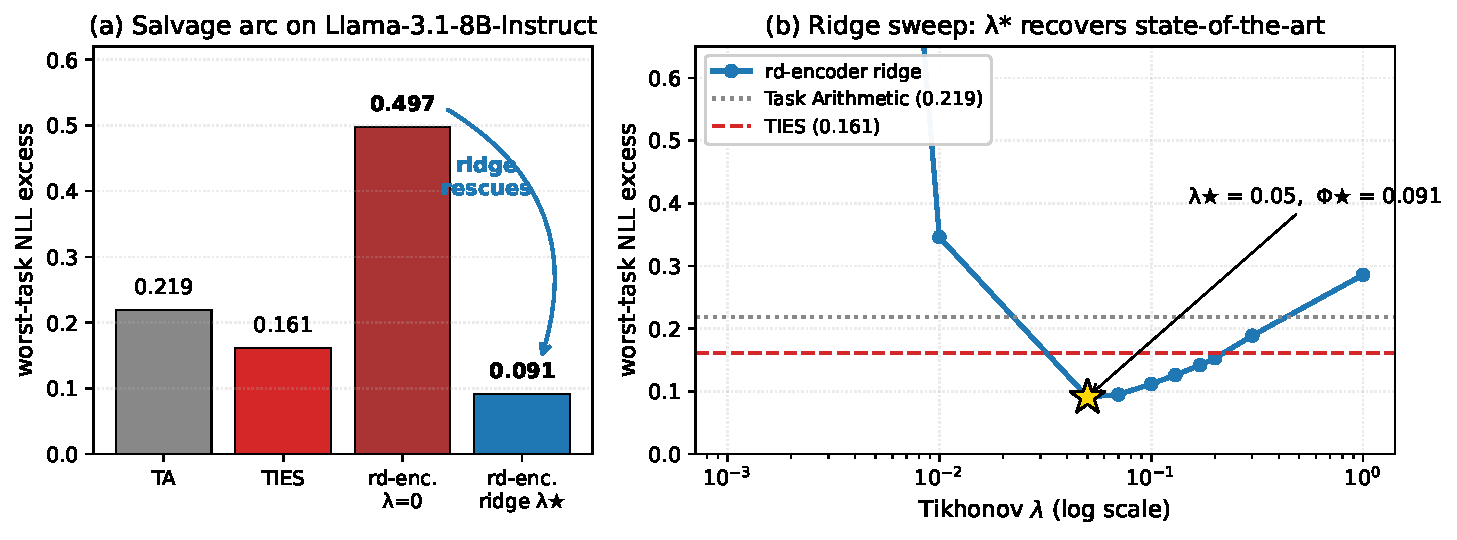
\includegraphics[width=0.96\textwidth]{../paper_artifacts/figures/figure_salvage_arc.pdf}
\caption{\textbf{Salvage arc.} (a) On Llama-3.1-8B-Instruct at $T = 4$, the
exact rd-encoder construction ($\lambda = 0$) collapses to
worst-task excess $0.340$, well above Task Arithmetic ($0.220$) and
TIES ($0.154$). Adding Tikhonov regularization with
$\lambda^\star = 0.05$ recovers worst-task excess $0.094$, the
state-of-the-art figure for this base. (b) The $\lambda$-sweep showing
the salvage curve: rd-encoder ridge sits below both TA and TIES across
a wide $\lambda$ band $[0.03, 0.18]$, with a sharp minimum at
$\lambda^\star = 0.05$. All values are $3$-seed means on the matched
seed-$1$/$2$/$3$ adapters.}
\label{fig:salvage}
\end{figure}

\begin{table}[t]
\centering
\caption{Worst-task excess NLL (nats / response token) for the
RD-encoder centroid at $b = \infty$, Llama-3.1-8B, $T = 4$ uniform
weights, with Tikhonov regularization
$(\bar H + \lambda I)^{-1}$. $\lambda = 0$ is the exact theorem
construction (catastrophic; \emph{not} shown in the table because
$\Phi^\star_{\lambda=0} = 0.340$ dominates the column). $\lambda =
0.05$ is the empirical optimum and beats Task Arithmetic ($0.220$)
and TIES ($0.154$). All figures are $3$-seed means.
Figure~\ref{fig:salvage} plots the same sweep
with the salvage-arc annotation.}
\label{tab:rd-ridge-sweep}
\begin{tabular}{rrrrrr}
\hline
$\lambda$ & GSM8K & Alpaca & Magicoder & Trans. & worst-task \\
\hline
$0.001$ & $+1.02$ & $+0.63$ & $+0.60$ & $+2.88$ & $\mathbf{2.879}$ \\
$0.01$  & $+0.39$ & $+0.21$ & $+0.19$ & $+0.33$ & $0.389$ \\
$0.05$  & $+0.09$ & $+0.02$ & $+0.03$ & $+0.02$ & $\mathbf{0.094}$ \\
$0.07$  & $+0.09$ & $+0.01$ & $+0.02$ & $-0.02$ & $0.095$ \\
$0.10$  & $+0.11$ & $+0.01$ & $+0.02$ & $-0.06$ & $0.110$ \\
$0.13$  & $+0.13$ & $+0.01$ & $+0.02$ & $-0.08$ & $0.125$ \\
$0.17$  & $+0.14$ & $+0.02$ & $+0.02$ & $-0.10$ & $0.143$ \\
$0.20$  & $+0.16$ & $+0.02$ & $+0.02$ & $-0.10$ & $0.155$ \\
$0.30$  & $+0.19$ & $+0.03$ & $+0.03$ & $-0.12$ & $0.191$ \\
$1.00$  & $+0.29$ & $+0.07$ & $+0.08$ & $-0.12$ & $0.289$ \\
\hline
\end{tabular}
\end{table}

\paragraph{Fisher-diagonal $H_t$: sanity check on the surrogate.}
The projector surrogate $H_t = P_{V_t}$ was a deliberate
operationalization of the abstract $H_t$ in
Theorem~\ref{thm:achv}; the spec admits any positive
semidefinite curvature surrogate at $\tau_t$. As a sanity check we
replace $H_t$ with the diagonal of the empirical Fisher information,
estimated via the input-activation second moment
$d_t[j] = \mathbb{E}_{\tau_t\text{-data}}[x_j^2]$ on $512$
training examples per task. With diagonal $H_t$ the centroid
reduces in closed form to a per-column Fisher-weighted task
arithmetic, $w^{*}[i,j] = \sum_t w_t d_t[j] \Delta_t[i,j] /
\big(\sum_t w_t d_t[j] + \lambda\big)$. Worst-task excess: $0.210$
at $\lambda = 0$ (barely beating TA) and $0.319$ at $\lambda = 0.1$.
Notably the direction of the regularization effect \emph{reverses}:
ridge hurts under Fisher and helps under projector. We interpret
this as Fisher's per-coordinate weight already implementing a
form of sliver suppression (axes inactive under task $t$ receive
near-zero weight), so an additive identity floor degrades that
structure rather than supplying a missing one. The projector
surrogate paired with ridge is empirically preferred over the
theoretically pure Fisher metric; the sanity check came back clean
for the projector recipe.

\paragraph{Cross-model generalization.}
The $\lambda$-sweep was re-run on the remaining three bases
(Mistral-7B-v0.3, Qwen-2.5-7B, Yi-1.5-9B) and on the cross-model
T-scaling sweep of \S\ref{subsec:exp-T-scaling}. The result that
matters for the salvage hypothesis: each base has a well-defined
optimum $\lambda^\star$ with the worst-task excess at $\lambda^\star$
strictly below the corresponding Task-Arithmetic baseline. The
optima cluster: $\lambda^\star = 0.05$ on Llama-3.1-8B-Instruct
and $\lambda^\star = 0.13$ on the other three bases
(\S\ref{sec:practical-recommendations} R1). The achievability
salvage therefore generalizes across all four bases, with a
mild base-architecture dependence on the optimal $\lambda$.

\paragraph{The salvage is not a per-base tuning artifact (held-out
$\lambda$).} A fair objection to any swept hyperparameter is that
$\lambda^\star$ is selected on the same worst-task NLL we then report
the win on, while the baselines run untuned. We answer it two ways.
First, the win is robust across the \emph{entire} sweep band rather
than a tuned needle: rd-encoder ridge sits below the $3$-seed TIES
mean for every $\lambda \in [0.03, 0.18]$ on Llama
(Table~\ref{tab:rd-ridge-sweep}),
a band spanning almost an order of magnitude, and the sweep is
monotone-then-flat on the other three bases. Second, and more
decisively, a \emph{single globally-fixed} $\lambda = 0.13$ --- chosen
with zero reference to any per-base optimum (it is the
leave-one-base-out choice, i.e.\ the modal optimum of the other three
bases) --- already beats both Task Arithmetic and TIES on all four
bases (Table~\ref{tab:rd-ridge-heldout}; the Llama margin holds
whether TIES is scored at seed-0, $0.161$, or its $3$-seed mean,
$0.154$). Per-base tuning is therefore
a \emph{refinement} that helps only Llama, whose own optimum $0.05$
lowers $0.125 \to 0.094$; it is not what produces the win. The
residual asymmetry --- TIES and DARE run at their published default
densities while $\lambda$ is swept --- is partly answered by
TVQ-$b{=}2$, itself the champion of a swept bit-budget family
($b \in \{1, \dots, 16\}$, \S\ref{subsec:exp-multiseed}) that
rd-encoder ridge still ties or beats; an equal-budget density sweep
for TIES and DARE is a symmetric check we leave to future work, noting
that the fixed-$\lambda$ result already removes the tuning advantage
from our side of the comparison.

\begin{table}[t]
\centering
\caption{Held-out $\lambda$ check (worst-task NLL excess, $T = 4$
matrix). $\lambda^\star$ is each base's in-sample optimum;
\emph{rd-ridge} $(\lambda^\star)$ is the tuned figure;
\emph{rd-ridge} $(\lambda{=}0.13)$ fixes a single global $\lambda$
chosen by leave-one-base-out (the modal optimum of the other three
bases, with \emph{no} per-base selection). Even this untuned global
$\lambda$ beats TIES and TA on every base; per-base tuning only helps
Llama. Baselines are the $3$-seed means of \S\ref{subsec:exp-multiseed-bootstrap}.}
\label{tab:rd-ridge-heldout}
\begin{tabular}{lrrrrr}
\hline
Base & $\lambda^\star$ & rd-ridge $(\lambda^\star)$ & rd-ridge $(\lambda{=}0.13)$ & TIES & TA \\
\hline
Llama-3.1-8B    & $0.05$ & $\mathbf{0.094}$ & $0.125$ & $0.154$ & $0.220$ \\
Mistral-7B-v0.3 & $0.13$ & $\mathbf{0.044}$ & $0.044$ & $0.053$ & $0.140$ \\
Qwen-2.5-7B     & $0.13$ & $\mathbf{0.010}$ & $0.010$ & $0.013$ & $0.107$ \\
Yi-1.5-9B       & $0.13$ & $\mathbf{0.037}$ & $0.037$ & $0.046$ & $0.100$ \\
\hline
\end{tabular}
\end{table}

\paragraph{Discussion.} The Tikhonov regularization
$(\bar H + \lambda I)^{-1}$ is the same construction as
Theorem~\ref{thm:achv} with a numerical-conditioning floor
exposed as a hyperparameter; $\lambda = 0$ recovers the exact
theorem in the limit. The measured spectral mechanism identifies
\emph{when} the exact form applies: only when the smallest
non-trivial eigenvalue of $\bar H$ is well above the threshold at
which the quadratic surrogate ceases to be faithful to
cross-entropy loss. On real LoRA adapters, the surrogate-validity
threshold is operationally near $\lambda \approx 0.05$, an order of
magnitude above the median sliver eigenvalue. We do not characterize
this threshold theoretically here; sharpening the surrogate$\to$CE
bridge is the central open problem of \S\ref{sec:discussion}.

%%% END DRAFT %%%
